\chapter{Datenbeschaffung und Datenspeicherung}\label{ch:data}

\section{Ausgangslage}

Um eine Zusammenstellung verschiedener Audiosegmente möglichst genau und inhaltlich abgestimmt auf ein bestimmtes Thema zu fokussieren, müssen auch zu diesem Thema passende Audioabschnitte in den Daten verfügbar sein.
Als Audiodaten könnten fast alle Audioressourcen genutzt werden, wie zum Beispiel Beiträge aus Radioprogrammen, die Audiospuren von Videos oder ganze Podcast Episoden.

Die Qualität dieses Systems würde mit steigender Anzahl an Audiomaterial bessere Ergebnisse erzielen, da dann zu vielen Themen mehr Inhalte zur Verfügung stehen.
Allerdings ist es im Umfang dieser Arbeit nicht möglich, alle verfügbaren Audiomaterial für die Erstellung der Podcasts zu verwenden.
Die Audiodaten müssten dazu erst transkribiert werden und anschließend mit diesen Transkripten Embeddings generiert werden, was Zeit- und Ressourcenintensiv ist.
Für diese Arbeit wurde versucht möglichst qualitativ hochwertige Daten zu benutzen, um mit den möglichen Ressourcen und in gegebener Zeit einen qualitativ hochwertigen Prototypen zu erstellen. 

Als Audiomaterial würde sich am besten Podcasts eignen, in denen über verschiedene Themen sachlich gesprochen wird, die Informationen aber gleichzeitig faktisch korrekt wären.
Außerdem sollten die Audioquellen frei verfügbar sein, damit keine Urheberrechtsverletzung stattfindet.

% Eine Garantie für Sachlichkeit und 

% Es sollten nicht die Vortragenden Personen wichtig sein  und sie nicht emotional oder persönlich 
% Als Audioquelle kommen vor allem wissensbasierte Podcasts in Frage, 
% Wissensbasierte Podcasts bieten als Audioform die besten qualitativen Inhalt für die Audiosegmente, wenn sie 

% Als Anbieter von Audiomaterial bieten sich zum Beispiel YouTube oder Spotify an, die sehr viele 


% Für die Grundlage der Audiosegmente bieten sich insbesondere wissensbasierte Podcasts an, die den Zuhörenden Informationen vermitteln wollen, wenn sie 


% Videos wie zum Beispiel von Youtube, setzen oft vorraus, dass der Zuschauer auch das Videomaterial sehen kann und somit würde nur das Hören der Audiospur zu verwirrung führen.

% Die Podcastbranche wächst seit vielen Jahren stetig und immer mehr Menschen hören regelmäßig Podcasts.
% In Deutschland schon über 29\%.


\section{Die ARD-Audiothek}

Die ARD-Audiothek ist in Deutschland eine der gößten Audio- und Podcastanbieter mit mitlerweile über 41 Millionen Audioabrufen und über 100.000 verschiedenen verfügbaren Audioinhalten. 
ALle Inhalte unterliegen den journalistischen Grundsätzen der ARD und bieten somit einen sorgfältigen Qualitätsstandard. 
Die verschiedenen Audioinhalte stammen von den einzelnen Landesrundfunkanstalten, der ARD und dem Deutschlandradio und liefern eine Vielzahl verschiedener Inhalte.
Sie enthält über 2000 verschiedene Podcasts, in vielen unterschiedlichen Kategorien, wie Comedy, Sport, Wissenschaft, Wirtschaft, Gesellschaft, Kunst, Musik oder Philosophie. 
In dieser Audiothek gibt es zudem Hörbücher, Hörspiele, oder Podcasts nur für Kinder.
Die einzelnen Rundfunkanstalten tragen außerdem eigene Podcasts bei, die meist einen regionalen Kontext haben, wie zum Beispiel der Podcast "Giga Grünheide" über das Teslawerk in Brandenburg vom rbb.
Alle diese Inhalte sind kostenlos und frei verfügbar und stellen eine gute Quelle für das Audiomaterial dar, das in dieser Arbeit verwendet wird.




% Im Appstore und im Google Playstore hat die App der ARD-Audiothek jeweils über eine Million Downloads.
% \cite{gotting2023}




\section{Podcastreihe Radiowissen}

Zur automatischen Generierung von Podcast Episoden bietet es sich an, dass in den Ausgangsaudios die Sprache klar und verständlich ist und verschiedene Sprecher sich nicht ins Wort fallen bzw. gleichzeitig reden.
Außerdem ist es wünschenswert, die ausgeschnittenen Audiosegmente an klaren Satzgrenzen zu teilen, sodass der Ausschnitt nicht mitten im Satz beginnt und dem Zuhörenden der Kontext vorenthalten wird. 

Aufgrund dieser Kriterien wurde als Datengrundlage die Podcastreihe Radiowissen von bayern2 benutzt. 
Diese ist nicht wie ein klassischer Podcast im Dialogstil aufgebaut, sondern ähnlich wie bei einem Hörspiel wird der Text von einem Manuskript abgelesen. 
Dazu kommen verschiedene Geräusche und verschiedene Stimmen, um dem Hörenden mehr Abwechselung zu bieten.

Der Fokus der einzelnen Episoden liegt auf interessanten Beiträgen zu verschiedenen Themen, die häufig Gebiete der Geschichte, Naturwissenschaft, Gesellschaft oder Philosophie umfasst.
Beispielepisoden sind: "Fasten - Verzicht und innerer Gewinn?", "Die Maus - Anpassungskünstler und gefürchteter Schädling", oder "Maria Sibylla Merian - Naturforscherin und Künstlerin".

Die mehr als 2000 Episoden wurden von mehr als 150 verschiedenen Autoren geskriptet.
Dadurch sind die einzelnen Episoden unterschiedlich in der Erzählweise.
In einigen Episoden kommen originale Audiospuren von historischen Aufnahmen vor oder auch  Gastbeiträge von Experten. Zudem wird beinahe jeder Podcast abwechselnd von mehreren Stimmen vorgetragen, was nachweislich die Aufmerksamkeit von Zuhörenden verbessert \cite{kang2012}.

\section{Datenbeschaffung über die ARD-Audiotheks API}

Die Inhalte der ARD-Audiothek kann man entweder direkt über die Webseite erreichen oder mithilfe einer frei benutzbare Web-GraphQL API abfragen.
(https://api.ardaudiothek.de/graphql) 
Über diese Schnittstelle sind alle Informationen, wie Titel, Beschreibungen, Autoren oder auch der Link zu dem MP3-File jeder Episode abrufbar.

Mit einer GraphQL-Abfrage \autoref{ch:graphql-1} erhält man alle Download-Links zu den Podcast-Episoden des Podcasts "Radio Wissen" von bayern2.
Das sind (Stand 3. Januar 24) 2257 Podcast Episoden.

Alle diese Audiodatein wurden anschließend heruntergeladen und auf einer lokalen Festplatte gespeichert.
Dabei kam es insgesamt 15-mal vor, dass zwei Episoden denselben Titel tragen, aber eine unterschiedliche Download-URL aufwiesen.
Die Download-URLs unterscheiden sich nur, indem am Ende die Zeichen "-1" oder "-2" angefügt wurden.
Zum Beispiel hat die Episode "Quantenphysik - Wahr, aber verrückt" den Downloadlink https://media.neuland.br.de/file/1804047/c/feed/quantenphysik-wahr-aber-verrueckt.mp3 aber auch https://media.neuland.br.de/file/2069613/c/feed/quantenphysik-wahr-aber-verrueckt-1.mp3.
In diesem Fall liefert nur die zweite URL einen Download, die erste zeigt eine Fehlermeldung an.
Es gibt auch Fälle in denen beide Links funktionieren, wie zum Beispiel 
https://media.neuland.br.de/file/32891/c/feed/die-bamberger-hexenprozesse-unschuldig-muss-ich-sterben.mp3 und
https://media.neuland.br.de/file/1858845/c/feed/die-bamberger-hexenprozesse-unschuldig-muss-ich-sterben-1.mp3 
Die Daten wurden dementsprechend bereinigt und doppelte Audioinhalte nur einmal abgespeichert.

Für weitere Analysen und die Kategorisierung der Audiodatein ist es außerdem Sinnvoll, die Beschreibungen der einzelnen Episoden und die dazugehörenden Schlagwörter abzufragen, da diese eine kurze Zusammenfassung oder Einordnung der Episoden enthalten.
Außerdem bietet das Entstehungsdatum der Episoden die Möglichkeit, Informationen später nach Aktualität zu filtern.
Über die Anfrage \autoref{ch:graphql-2} können all diese Informationen abgefragt werden.

Über die API kann auch in einigen Fällen direkt ein Transkript des Audiofiles angefordert werden. 
Allerdings ist die Transkription meist nicht sehr akkurat.
Nähreres dazu in Kapitel \autoref{ch:method}


\section{Datenanalyse}


Die 2232 einzigartigen Episoden haben eine durchschnittliche Länge von 22 Minuten und eine durchschnittliche Größe von 21 MB.
Insgesamt weisen diese Audiodaten eine Größe von ungefähr 47 GB auf. 

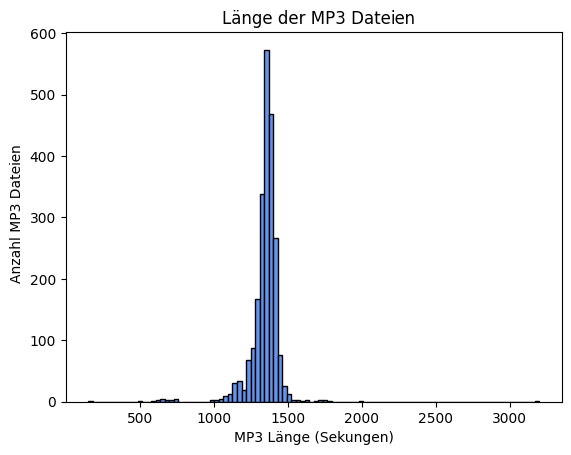
\includegraphics[width=\linewidth]{figures/mp3_length.png}

Der Graph zeigt die Verteilung der Längen der Audiodatein.

Der kürzeste Podcast ist "ab-jetzt-in-der-ard-audiothek-kinder-der-flucht-frauen-erzaehlen.mp3", der nur 2 Minuten 30 Sekunden lang ist und ein Teaser für einen anderen Podcast darstellt.
Die längste MP3 Datei ist mit Abstand "deportation-und-exil-eine-polnische-odyssee-im-zweiten-weltkrieg.mp3" mit einer Länge von mehr als 53 Minuten.
Diese Episode ist mehr als doppelt so lang wie eine durchschnittliche Episode und bildet einen Ausnahmefall.

Für das System werden trotz der verschiedenen Längen alle Audiodatein benutzt, da sie später in kleinere Segmente zerteilt werden.



\section{Transkription der Podcasts (ASR)}


\subsection{Fraunhofer}

Seit 2015 arbeitet die ARD mit dem Fraunhofer-Institut Institut für Intelligente Analyse- und Informationssysteme (IAIS) zusammen, um „Erschließung von Mediendaten zu forcieren und dabei den Schwerpunkt auf maschinelle Verfahren zu legen“ [1]
Ein Teil dieses Projektes bezieht sich auf das Audio-Mining. 
Das Fraunhofer IAIS entwickelte dafür ein System, welches die Audiodatein transkribiert und dabei „in der kompletten ARD, bei Deutschlandradio sowie im ZDF im Einsatz [ist]“. 
Leider legt das FraunhoferIAIS nicht offen, welche Technologie es dafür verwendet. 
Die Transkripte lassen sich allerdings sehr einfach über eine Graphql Schnittstelle abfragen. 

\subsection{Microsoft Translate}

Eine weitere Möglichkeit zur Audiotranskription bietet Microsoft Translate. 
Soweit man einen Microsoft 365 Account besitzt, kann man in dem Webinterface von Microsoft word eine Transkriptionsfunktion benutzen. 
Dafür müssen die Audiofiles zunächst auf Microsoft Onedrive hochgeladen werden und können dann mit einem Klick übersetzt werden. 
Microsoft Word stellt dann sogar Timestamps  zur Verfügung für das ganze Dokument. 
Die Qualität ist außerdem besser als bei kostenlosen Open-Source Alternativen. 
Dafür skaliert diese Art der Transkription schlecht für größere Datenmengen, da sämtliche files zunächst bei OneDrive hochgeladen werden müssen und dann jedes File von Hand ausgewählt, in Word eingebunden, transkribiert werden und dann abgespeichert werden müssen. 

\subsection{Whisper}

Für die Transkription eignen sich Automatic Speech Recognition Systeme (ASR). 
Eines der besten kostenlosen ASR Systeme bietet Whisper von OpenAI. 
Dieses System wurde mit einem maschinellen lernverfahren auf 680 000 Stunden Audiomaterial in verschiedenen Sprachen trainiert. 
Es ist sehr leistungsstark und kann lokal auf eigener Hardware laufen. [2] [3]

Whisper bietet mehrere verschiedene Modelle zur Transkription an. Es gibt die Modelle tiny, base, small, medium und large. 
Das Basismodell hat ca. 74 Millionen Parameter und benötigt ca. 1 GB VRAM und ist ca. 16 mal schneller als das large Model. 
Bei einem Test für die Episode 1968-das-ausnahmejahr aus dem Podcast Radiowissen von br2 schneidet es aber nicht sehr gut ab. 
Aus dem Wort „Vietnam“ wird „Wirdnam“, aus „Panzer in Prag“ wird „Panzer-Inprac“ und aus  „Ohrfeige“ wird „Urfeige“. 
Der vorgetragene Text wurde dabei ohne Störgeräusche und von einer Person flüssig vorgetragen. 

Dagegen bietet das Medium Model von Whisper deutlich bessere Ergebnisse für die selbe Episode. 
Bei der Transkription konnte kein Fehler festgestellt werden. Allerdings ist der Zeitaufwand durch höhere Rechenleistung immens. 
Auf einem Macbook Pro 2016 mit einem Intel Core i7 benötigt die Transkription ca. 45 min. pro Episode. 
Auf einer T4 GPU, wie sie Google kostenlos auf Google Colab zur verfügung stellt, dauert eine Transkription immer noch 3,5 Minuten. 
Für ca. 1000 Episoden bräuchte man demnach ca. 3500 Minuten, d.h. ca. 58 h. 

Drawbacks von Whisper:
Medium Modell immer noch einige Fehler: 
- gubt statt Grub
- wenn Sprecherwechsel manchmal ganze Sätze weg (im-bann-des-mondes-archaische-mythen-und-religionen.mp3	)

TODO large ausprobieren, auf den Servern der Uni und mit der Ebu API
Eurovox


Die Transkripte der Episoden sind meißt ca. 3000 Wörter lang und benötigen ungefähr 20 KB Speicherplatz pro Transkript.

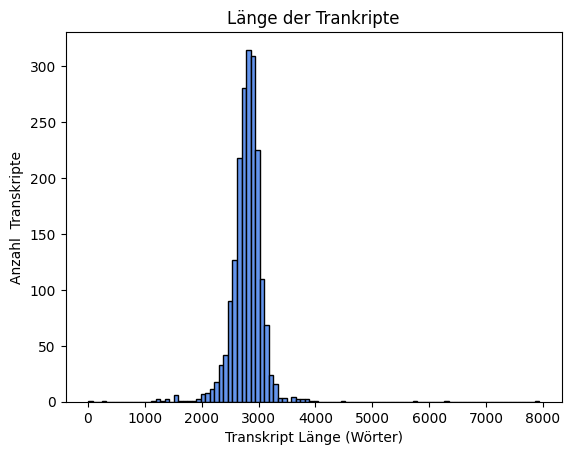
\includegraphics[width=\linewidth]{figures/transcript_length.png}


\subsection{Eurovox}

Das Problem der langen Wartezeiten lässt sich umgehen, wenn wir Cloud computing benutzen, das heißt, das Whisper model nicht auf der lokalen Hardware laufen zu lassen, sondern zum Beispiel auf den Servern von Eurovox. 
Eurovox ist ein Software tool von der EBU, der Europian Broadcast Union. 
Sie ist ein zusammenschluss von derzeit 68 Rundfunkanstalten in 56 Staaten Europas, Nordafrikas und Vorderasien mit Sitz in Genf. [4] 
Das tool Eurovox steht dabei allen Mitgliedern zur Verfügung.  
Mithilfe dieses Tools kann man Text-to-Speech, Übersetzungen und Speech-to-Text Services über eine UI benutzen. 
Es gibt sogar die Möglichkeit wärend eines Streams live audio captions zu erzeugen. 
Für dieses Projekt benutzen wir aber zunächst nur die Translation Funktion. 
Außerdem verwenden wir die API von Eurovox um später das ganze Projekt auf mehr Episode Transkripte ausweiten zu können. 
Laut den Entwicklern soll die API auch demnächst open-sourced werden [QUELLE].

Die API stellt, ebenso wie das Tool, eine Reihe verschiedener Anbieter zur verfügung, über die wir die Audios transkribieren lassen können. 


\section{Embedding erstellung}



\section{Datenaufbereitung}

\subsection{Satzbildung}

Die transkribierten Daten, welche Whisper erzeugt enthalten die erkannten Wörter, sowie die einzelnen Zeitstempel für den Start und das Ende jedes Wortes mit einer genauigkeit von Zehntelsekunden.
Für die spätere Analyse der Daten, ist es Sinnvoll die einzelnen Wörter in größere Segmente zusammenzufassen, damit bei einer Suchfunktion der Kontext von erschiedenen Wörtern miteinbezogen werden kann.

Für die Wahl der richtigen Segmentgröße gibt es keine einheitliche Lösung.
Da wichtige Informationen über mehrere Sätze verteilt liegen können, kann es bei einfacher segmentierung zu dem Problem kommen, dass die Information in zwei Segmente gestückelt wurde.
Um dem entgegenzuwirken ist es sinnvoll, die einzelnen Segmente überlappend zu erstellen.

Ein naheliegender Ansatz besteht darin, die einzelnen Wörter zunächst in Sätze zu gruppieren.
Für diese Gruppierung werden zwei Ansätze betrachtet.
Der einfachste Ansatz besteht darin, die von Whisper erzeugten Satzpunkte als  Trennzeichen für einen Satz zu zählen.
Whisper erkennt von sich aus aufgrund der Tonlage und der Pause zwischen Wörtern und der grammatikalischen Struktur der vorangegangenen Wörtern, ob ein Wort das Ende eines Satzes markiert. ???
Dann gibt Whisper das Wort mit einem Punkt, einem Fragezeichen, oder einem Ausrufezeichen am Ende als erkanntes Wort aus.
Diese Punktuation kann man benutzen, um die einzeln Wörter in Sätze zu gruppieren.
Leider ergibt sich dabei das Problem, dass bestimmte Wörter, oder Abkürzungen zusätzöiche Punkte enthalten.
Beispiele sind "Mr. Smith", "seinem 26. Studioalbum", "am 10. Januar 2016".
Mit diesem naiven Ansatz der Satztrennung, würden wir also einige Sätze an ungewollten Stellen in mehrere Sätze auftrennen.

Um dieses Problem zu lösen, muss der Algorithmus verstehen, welche Satzzeichen die wirklichen Satzenden sind.
Dies erfordert ein verständnis der Satzstruktur und ist deswegen nicht trivial möglich.
Um die Sätzegrenzen zu finden, wird deshalb die Open-Source Sprachbibliothek SpaCy.\cite{honnibal2017}

David Bowie stirbt am 10. Januar 2016 an Leberkrebs.
Zwei Tage nach seinem 69. Geburtstag und der Veröffentlichung von Blackstar, seinem 26. Studioalbum.

\subsection{Satzbildung mit SpaCy}

Mithilfe der NLP Bibliothek SpaCy kann man herausfinden, welche Satzzeichen wirklich die Grenze eines Satzes Markieren.
SpaCy verwendet dafür Machine Learning Modelle, die aufgrund von vielen Daten gelernt haben, wo das Ende eines Satzes ist.
Es gibt auch noch die beliebte Bibliothek NLKT, die sich aber eher auf das Unterrichten von NLP spezialisiert hat.
SpaCy ist eher für den produktiven Einsatz geeignet.
Auf der offiziellen Webseite von spaCy werden vier verschiedene Modelle für die deutsche Sprache zur verfügung gestellt.
Das Modell 
\begin{verbatim}
    de_core_news_sm 
\end{verbatim} 
ist das kleinste Modell mit 13 MB Größe, dann folgt 
\begin{verbatim} 
    de_core_news_md 
\end{verbatim}
mit einer Größe von 42 MB und 
\begin{verbatim}
    de_core_news_lg 
\end{verbatim}
ist das größte Modell mit 541 MB.
Das größte Modell bietet dabei vor allem viele vortrainierte Embedding Vektoren für einzelne Wörter.
Das vierte Modell ist 
\begin{verbatim}
    de_dep_news_trf
\end{verbatim}
verbraucht 391 MB Speicherplatz und ist speziell für Transformer-support geeignet.
spaCy führt eine selbst angegebenen Accuracy Evaluation für Sentence Segmentation, also das Erkennen von Satzenden in einem Text.
Darin ist der F-Score für das kleine Modell gleich 0,94; für das mittlere Modell 0,95 und für das große Modell ebenfalls 0,95.
Das Modell mit der Transformer pipeline bietet einen F-score von 0,98 und wird deswegen in dieser Arbeit verwendet. \cite{spacy2024}




\subsubsection{Embeddings}

\subsection{Ählichkeitssuche lexikalisch}

\subsubsection{Keywordsuche}

Eine Möglichkeit bietet sich in der Keywordsuche. 
Hierbei wird einfach überprüft, ob sich ein Keyword in einem der Dokumente wiederfindet. Ist die möchte ein User beispielsweise einen zusammengeschnittene Podcast Episode über „Zugspitze“, so schaut das System, in welchen Episodensegmenten das Wort „Zugspitze“ auftaucht, und gibt diese zurück. 
Schwieriger wird es, wenn die Useranfrage mehrere Wörter beinhaltet. 
Möchte sich der User über das Thema „Zugspitze wandern“ informieren so müsste zunächst untersucht werden, welche Dokumente beide Worte enthalten, welche nur eines der beiden enthalten. 
Dann müsste man dementsprechend auch ein Algorithmus entwickeln, der diese dann sinnvoll hierarchisiert. 

\subsubsection{TF-IDF}

Einen solchen Ansatz bietet das TF-IDF Maß (Term Frequency – Inverse Document Frequency). 
Im Bereich des NLP verwendet man das TF-IDF Maß um zu untersuchen welche Wörter in verschiedenen Dokumenten welche Gewichtung erfahren. 
Dazu wird zunächst die TF-Matrix, also die Term Frequenzy Matrix berechnet. 
Hierbei wird erst das Vokabular ermittelt, also die Gesamtheit aller Tokens (Wörter) die es in allen Dokumenten (Transkript Segmenten) des Korpuses (alle heruntergeladenen Episoden) gibt. 
Dann wird für jedes einzelne Segment die Anzahl jeder in ihm auftretenden Tokens ermittelt. 
Für den Satz: „Auf der Zugspitze gibt es viele Wanderer, die die Zugspitze lieben“. 
In diesem Fall würde in der TF Matrix an der Stelle Zugspitze eine 2 Stehen, in der Zeile Wandern aber 0, da zwar das Wort Wanderer, aber nicht das Wort wandern vorkommt. 
Da diese beiden Worte aber sehr ähnlich sind und der User bei einer Anfrage nicht immer nach verschiedenen Versionen eines Wortes suchen will, um dann ein zufriedenstellendes Audio zu erhalten


\subsection{Sätze Normalisieren / cleanen}

Für Retrieval funktionen ist es Sinnvoll, mehrere Wörter zusammenzufassen.
Wenn man einen Algorithmus hat, der gezielt Wörter im Korpus suchen kann, ist es Wünschenswert nicht nur exakt die selben Wörter zu suchen, sondern auch verwandte Wörter.
Zum Beispiel sollte die Suche nach dem Wort "Wanderer" auch Ergebisse für die Worte "Wandererin", "Wanderung" oder "wandern" enthalten, nicht aber das Wort "Wand".

\subsubsection{Tokenisierer}

In Machine Leerning Anwendungen nutzt man dafür verschiedene Tokenisierer.
Es gibt einfache Tokenisierer, wie Whitespace Tokenisierer, die einen Text einfach an Leerzeichen teilen und die einzelnen Wörter als Tokens behandeln.
Etwas besser sind Wort Tokenizer, die auch Satzzeichen erkennen und dadurch Punkte und Kommata nicht an das Ende des vorangegangenen Wortes anhängen. 
Einen solchen Tokenizer nutzt beispielsweise spaCy, um "Linguistic Features" zu bestimmen.
Es gibt Subword tokenisierer, die Worte nocheinmal in kleinere Abschnitte teilen.
Das Byte-Pair Encoding versucht aufgrund von Statistischen Methoden, häufig vorkommende zusammenhängende Zeichenfolgen als Tokens zu identifizieren.
Diese Art Tokenizer wird zum Beispiel oft für die Eingabe bei Transformern genutzt. [Quelle]
Die Transformermodelle von OpenAI benutzen beispielsweise tiktoken als Tokenizer [Quelle], das BERT Modell von Google benutzt den WordPiece Tokenizer.



\subsubsection{Lemmatisierung vs. Stemming}

Um diese Abbildung von mehreren Worten auf ein Stammwort zu erreichen, gibt es zwei unterschiedliche Methoden:
Die Methode Stemming versucht regelbasiert Suffixe von Worten zu ersetzen, um aus Wörtern mit verschiedenen Endungen, wie zum Beispiel "Wanderer" und "Wanderung" zu einem Wort "Wander" zu reduzieren.
Der Vorteil ist, dass der Algorithmus sehr schnell agieren kann, um die Worte auf ihre Stammform zu reduzieren.
Die Nachteile sind allerdings, dass die Deutsche Sprache sehr viele verschiedene Wortkonstrukte erlaubt, die nicht alle mithilfe von einzelnen Regeln auf ein gemeinsammes Stammwort gebracht werden können. 
Zum Beispiel bei dem Plural von "Baum"; "Bäume".


\subsubsection{Kompositatrennung Pyphen vs german compound splitter}

Als weiteren Vorverarbeitungsschritt für die effiziente Keywordsuche kann man zusammengesetzte Wörter in ihre bestandteile auftrennen.
Das Vokabular des Datensazes besteht zu 61\% aus Nomen. 
Die meisten der Nomen sind zusammengesetzte Nomen, manche davon sind sehr lang, wie zum Beispiel "reichsdeputationshauptschlussakte", oder "hochgeschwindigkeitstransportmittel".
In dem ganzen Vokabular, das aus den Transkriptionen von Whisper stammt, besteht fast die Hälfte (47,8\%) aus zehn oder mehr Buchstaben.
Da für exakte Keywortsuche solche Begriffe fast nie auftreten, lohnt es sich, 



Dabei gibt es allerdings keine Möglichkeit, die verschiedenen Treffer dieser suche nach Relevanz zu hierarchisieren. Sucht man zum Beispiel nach dem Stichwort „Klimakrise“ würden dabei mehrere Stunden Material zusammenkommen [QUELLE]. 
Man könnte nun einfach die Ersten Segmente nehmen, die zusammen die vorgegebene Zeit überbrücken. Allerdings ist dieser Ansatz wenig Vielversprechend. 


\subsection{Embeddings Dense}

Dazu werden die einzelnen Sagmente mit den verschiedenen Modellen embedded.
Am Anfang des Segments kann noch einmal der Titel der Episode angefügt werden, was eventuell die Performance steigert.\cite{jones2021}


\section{Datenspeicherung}

\subsection{Datenspeicherung SQLite}

Für die Analyse werden die MP3-Dateien der einzelnen Podcast-Episoden in einem seperaten Ordner gespeichert und die Benennung der originalen Dateien stammt aus der Download-URL.
Zur Speicherung der Transkripte wird das relationale Datenbank Managment System (RDBMS) SQLite  eingesetzt. SQLite ist für Datenanalysezwecke sehr gut geeignet, weil es simpel und performant ist und als opensource-Projekt kostenlos verwendet werden kann.
Im Gegensatz zu anderen RDBMS, wie mySQL oder PostgreSQL arbeitet SQLite serverunabhängig und speichert alle Tabellen in einer einzigen Datei, was sehr nützlich für den Datenaustausch zwischen verschiedenen Geräten ist.
Für einige Operationen, wie die Transkription der Audiodateien oder die Generierung von Embeddings wird die Hardware eines High-Performance Clusters der Technischen Hochschule Nürnberg genutzt. 
Um die Daten zu analysieren und zu nutzen bietet es sich an, auf Consumer-Hardware zu wechseln und dafür ist eine gute Portabilität der Datenbank von Vorteil.

SQLite unterstützt Datenmengen bis zu 140 TB. 
Allerdings wird auf der offiziellen Webseite angegeben, dass ab einer Größe von 1 TB auf serverbasierte RDBMS umgestiegen werden sollte, da die gesamte Datenbank in einem File gespeichert wird und viele Client-Betriebssysteme eine maximale Größe der Dateien vorgeben. 
Falls das Projekt in der Zukunft auf mehrere Podcastreihen ausgeweitet wird, sollte vor diesem Hintergrund ein Wechsel des DBMS in Betracht gezogen werden.

\subsection{Datenspeicherung Vektoren SQLite}

Da SQlite nativ keine Listen oder Tabellen als Einträge in einer Datenbank speichern kann, ist es nicht trivial, die Embeddings abzuspeichern.
Zunächst wurde die Möglichkeit in Betracht gezogen, jeden einzelnen Eintrag aus einem Embedding-Vektor als seperaten Eintrag in einer Tabelle zu speichern. 

Das führt allerdings zu sehr ineffizienten Abfragen der Daten und beim Einfügen von Daten limitiert SQLite die Anzahl der Parameter, sodass längere Embeddings umständlich gestückelt abgespeichert werden müssten.

Als Nächstes wurde überprüft, ob man die Embeddings als serialisiertes Array abspeichern kann.
Dafür wurde jedes Embedding in einen JSON-String umgewandelt, der dann gespeichert werden soll. 
Dabei tritt leider das Problem auf, dass die Daten bei der Verwendung wieder deserialisiert werden müssen.
Dieser Schritt müsste jedes Mal wiederholt werden, wenn eine Suche stattfindet. 
Dies dauert sehr lange und ist sehr ineffizient. 
Für die deserialisierung von 400.000 Sätzen mit einem 384 dimensionalen Embedding eines Sentence Transformer Modells auf einem Intel i7 Quad-Core beträgt die Rechenzeit ca. 45 Min.

Zur Datenspeicherung der Embedding-Vektoren muss zwischen Dense- und Sparce-Vektoren unterschieden werden, da für beide Embedding-Methoden unterschiedliche Optimierungen in der Speicher und Retrival Funktionalität vorliegen. 

\subsection{Datenspeicherung Dense Vektoren}

Um Dichte-Vektoren abzuspeichern, bietet es sich an, eine seperate Vektordatenbank zu nutzen.
Eine Vektordatenbank ist eine nichtrelationale Datenbank, die darauf spezialisiert ist, eine effiziente Suche in ungeordneten Informationen zu ermöglichen.
Dazu speichert sie die Embedding-Vektoren verschiedener Datenquellen effizient ab und erlaubt Zugriff auf schnelle Suchalgorithmen, wie Approximate Nearest Neighbour Algorithmen.

Es gibt verschiedene Approximate Nearest Neighbour Algorithmen, die alle darauf abzielen, den gesamten Suchraum für eine Ähnlichkeitssuche in kleinere Unterräume aufzuteilen.
Dabei werden oft Baum-Strukturen verwendet, um die Suche effizienter zu gestalten.
Speziell Algorithmen wie Hierarchical Navigable Small Worlds werden von vielen Vektordatenbanken benutzt.

% Vektordatenbanken entwickeln sich in den letzten Jahren stark weiter.
% In diesem Projekt wurde zunächst die Vektordatenbank Milvus betrachtet.
% Milvus kann sehr gut auf große Datenmengen skalieren und wird deshalb in vielen großen Unternehmen, wie Nvidia, Paypal oder ebay eingesetzt. 
% Außerdem bietet Milvus Unterstützung für eine clusterbasierte Struktur, in der einzelne Container dynamisch zusammenarbeiten können. 
% Dadurch wird eine gute Skalierbarkeit für große Datenmengen erreicht. 
% Für kleinere Projekte ist der Setup-Aufwand sehr groß und die Lernkurve sehr steil.

% Pinecone, Zilliz, Qdrant

% Außerdem gibt es eine Erweiterung für die PostgreSQL Datenbank namens pg-Vector

% Die Vektordatenbank Redis

% Durch die Neuheit der Vektordatenbanken bedingt, gibt es kaum Vergleiche zwischen diesen.
% \cite{blueteamai}


% In dieser Arbeit wird die Vektordatenbank Milvus verwendet.
% Milvus ist eine Open-Source Vektordatenbank die von dem Unternehmen Zilliz entwickelt wird.
% Laut eigenen Angaben ist sie die am weitseten fortgeschrittene Vektordatenbank und wird von vielen Unternehmen, wie Nvidia, Paypal oder ebay benutzt.

In dieser Arbeit wird die Vektordatenbank Chroma verwendet. 
Chroma ist eine einfache Vektordatenbank, die die Daten sowohl lokal als auch über eine Client-Server-Schnittstelle speichern kann.
Das Projekt ist erst im Mai 2022 als Start-up entstanden, verfügt aber mittlerweile über viele Features, die die Datenverwaltung erheblich vereinfachen.
Die Datenbank ist dabei mit einer NoSQL-Datenbank zu vergleichen, indem die Daten nicht relational in Tabellen gespeichert werden, sondern in einer Collection als Objekte mit verschiedenen Metadaten.
Jedes dieser Objekte hat eine Document-Eigenschaft, welche den Inhalt des Dokuments repräsentiert.
Dieser Inhalt ist in diesem Fall ein Ausschnitt aus einem Transkript, könnte aber auch ein Bild oder eine Audiodatei darstellen.

Außerdem besitzt jedes Objekt einen Embedding-Vektor, der mit dem Dokument assoziiert wird. 
Innerhalb einer Collection müssen alle Objekte mit derselben Embedding-Methode encodiert werden.
Das sichert die Vergleichbarkeit der verschiedenen Vektoren untereinander.

ChromaDB bietet nativen Support für verschiedene Embedding Modelle von OpenAI, Huggingface, Cohere, instructorembedding und JinaAI.
Dafür müssen nur das Model und der plattformspezifische API-KEY angegeben werden und Chroma erstellt automatisch für jedes Dokument das Embedding.
Standardmäßig ist das Embedding des Sentence Transformer Modells all-MiniLM-L6-v2 eingestellt.
Alternativ können auch schon vorgefertigte Embeddings eingefügt und die dazugehörige Embedding Funktion eingetragen werden.
In dieser Arbeit wurden die Embeddings von OpenAI und all-MiniLM-L6-v2 schon vorher erstellt und dort eingetragen.

Chroma bietet außerdem sehr guten Support für effizientes Retrieval von Dokumenten.
Dazu sind schon verschiedene verfahren der Nearest Neighbour Suche implementiert.
 

In diessem Projekt wurde erst in einer späten Phase der Umstieg auf die Vektordatenbank vollzogen, weshalb einige Funktionen, die in dieser Datenbank automatisch integriert sind, noch einmal sehr ausführlich beschrieben werden.


\subsection{Datenspeicherung Sparce Vektoren}

Chroma bietet leider noch keine Unterstützung zur Speicherung von Sparce Vektoren.
Stattdessen wurde das Python-Modul pickle verwendet, welches darauf spezialisiert ist, Python Objekte effizient als Bytecode zu serialisieren. 
Es bietet auch die Möglichkeit, Datenstrukturen effizient zu speichern bzw. zu laden und hat seit Python 3.8 auch guten Support, um große NumPy Arrays effizient zu speichern, was zuvor nur mit der joblib Bibliothek möglich war.
Pickle speichert die Daten in einem Python spezifischen Format ab, was die Portierbarkeit auf andere Systeme stark einschränkt. Dieses Format erlaubt es aber verschiedene Eigenschaften besser zu speichern als JSON (z.B. Pointer sharing).

Für den TF-IDF Algorithmus, bei dem ein Vokabular von mehr als 200.000 Wörtern eine ebensogroße Dimensionalität der Embeddingvektoren benötigt, würde ein normaler Serialisierungsalgorithmus für die 300.000 Sätze ca 60 Milliarden Werte abspeichern.
Wenn man für jeden dieser Werte eine 32 Bit Gleitkommazahl als Datentyp abspeichern würde, käme man auf ca. 240 GB Daten. 
Ein Großteil dieser Werte (~99,9\%) sind dabei 0.
Ein Numpy Array kann diese Werte sehr effizient zusammenfassen und mithilfe von pickle kann dieses kompakte Array effizient abgespeichert werden, wodurch eine tatsächliche Speichergröße von ca. 50 MB entsteht.
Dies ermöglicht auch ein effizientes laden und vergleichen der Embeddings, was für 400.000 Sätze auf einem Intel Quad-Core i7 ca. 1 Sekunde benötigt.

In der Zukunft könnte dieser Schritt durch einen Umstieg auf eine Plattform wie Elasticsearch vereinfacht werden.



% \subsection{weitere Schritte}


% Eine bekannte Bibliothek für Nearest Neighbour Searches ist Annoy, die unter anderem bei Spotify für die Recommendations von Songs verwendet wird. [Quelle]
% Eine weitere bekannte bekannte Bibliothek für Nearest Neighbour Searches ist FAISS (Facebook AI Similarity Search)

